%%%%%%%%%%%%%%%%%%%%%%%%%%%%%%%%%%%%%%%%%
% Friggeri Resume/CV
% XeLaTeX Template
% Version 1.0 (5/5/13)
%
% This template has been downloaded from:
% http://www.LaTeXTemplates.com
%
% Original author:
% Adrien Friggeri (adrien@friggeri.net)
% https://github.com/afriggeri/CV
%
% License:
% CC BY-NC-SA 3.0 (http://creativecommons.org/licenses/by-nc-sa/3.0/)
%
% Important notes:
% This template needs to be compiled with XeLaTeX and the bibliography, if used,
% needs to be compiled with biber rather than bibtex.
%
%%%%%%%%%%%%%%%%%%%%%%%%%%%%%%%%%%%%%%%%%

\documentclass[]{friggeri-cv} % Add 'print' as an option into the square bracket to remove colors from this template for printing

\addbibresource{bibliography.bib} % Specify the bibliography file to include publications

\begin{document}

\header{Arnaud}{Bletterer}{Etudiant en Informatique Graphique} % Your name and current job title/field

%----------------------------------------------------------------------------------------
%	SIDEBAR SECTION:
%----------------------------------------------------------------------------------------

\begin{aside} % In the aside, each new line forces a line break

%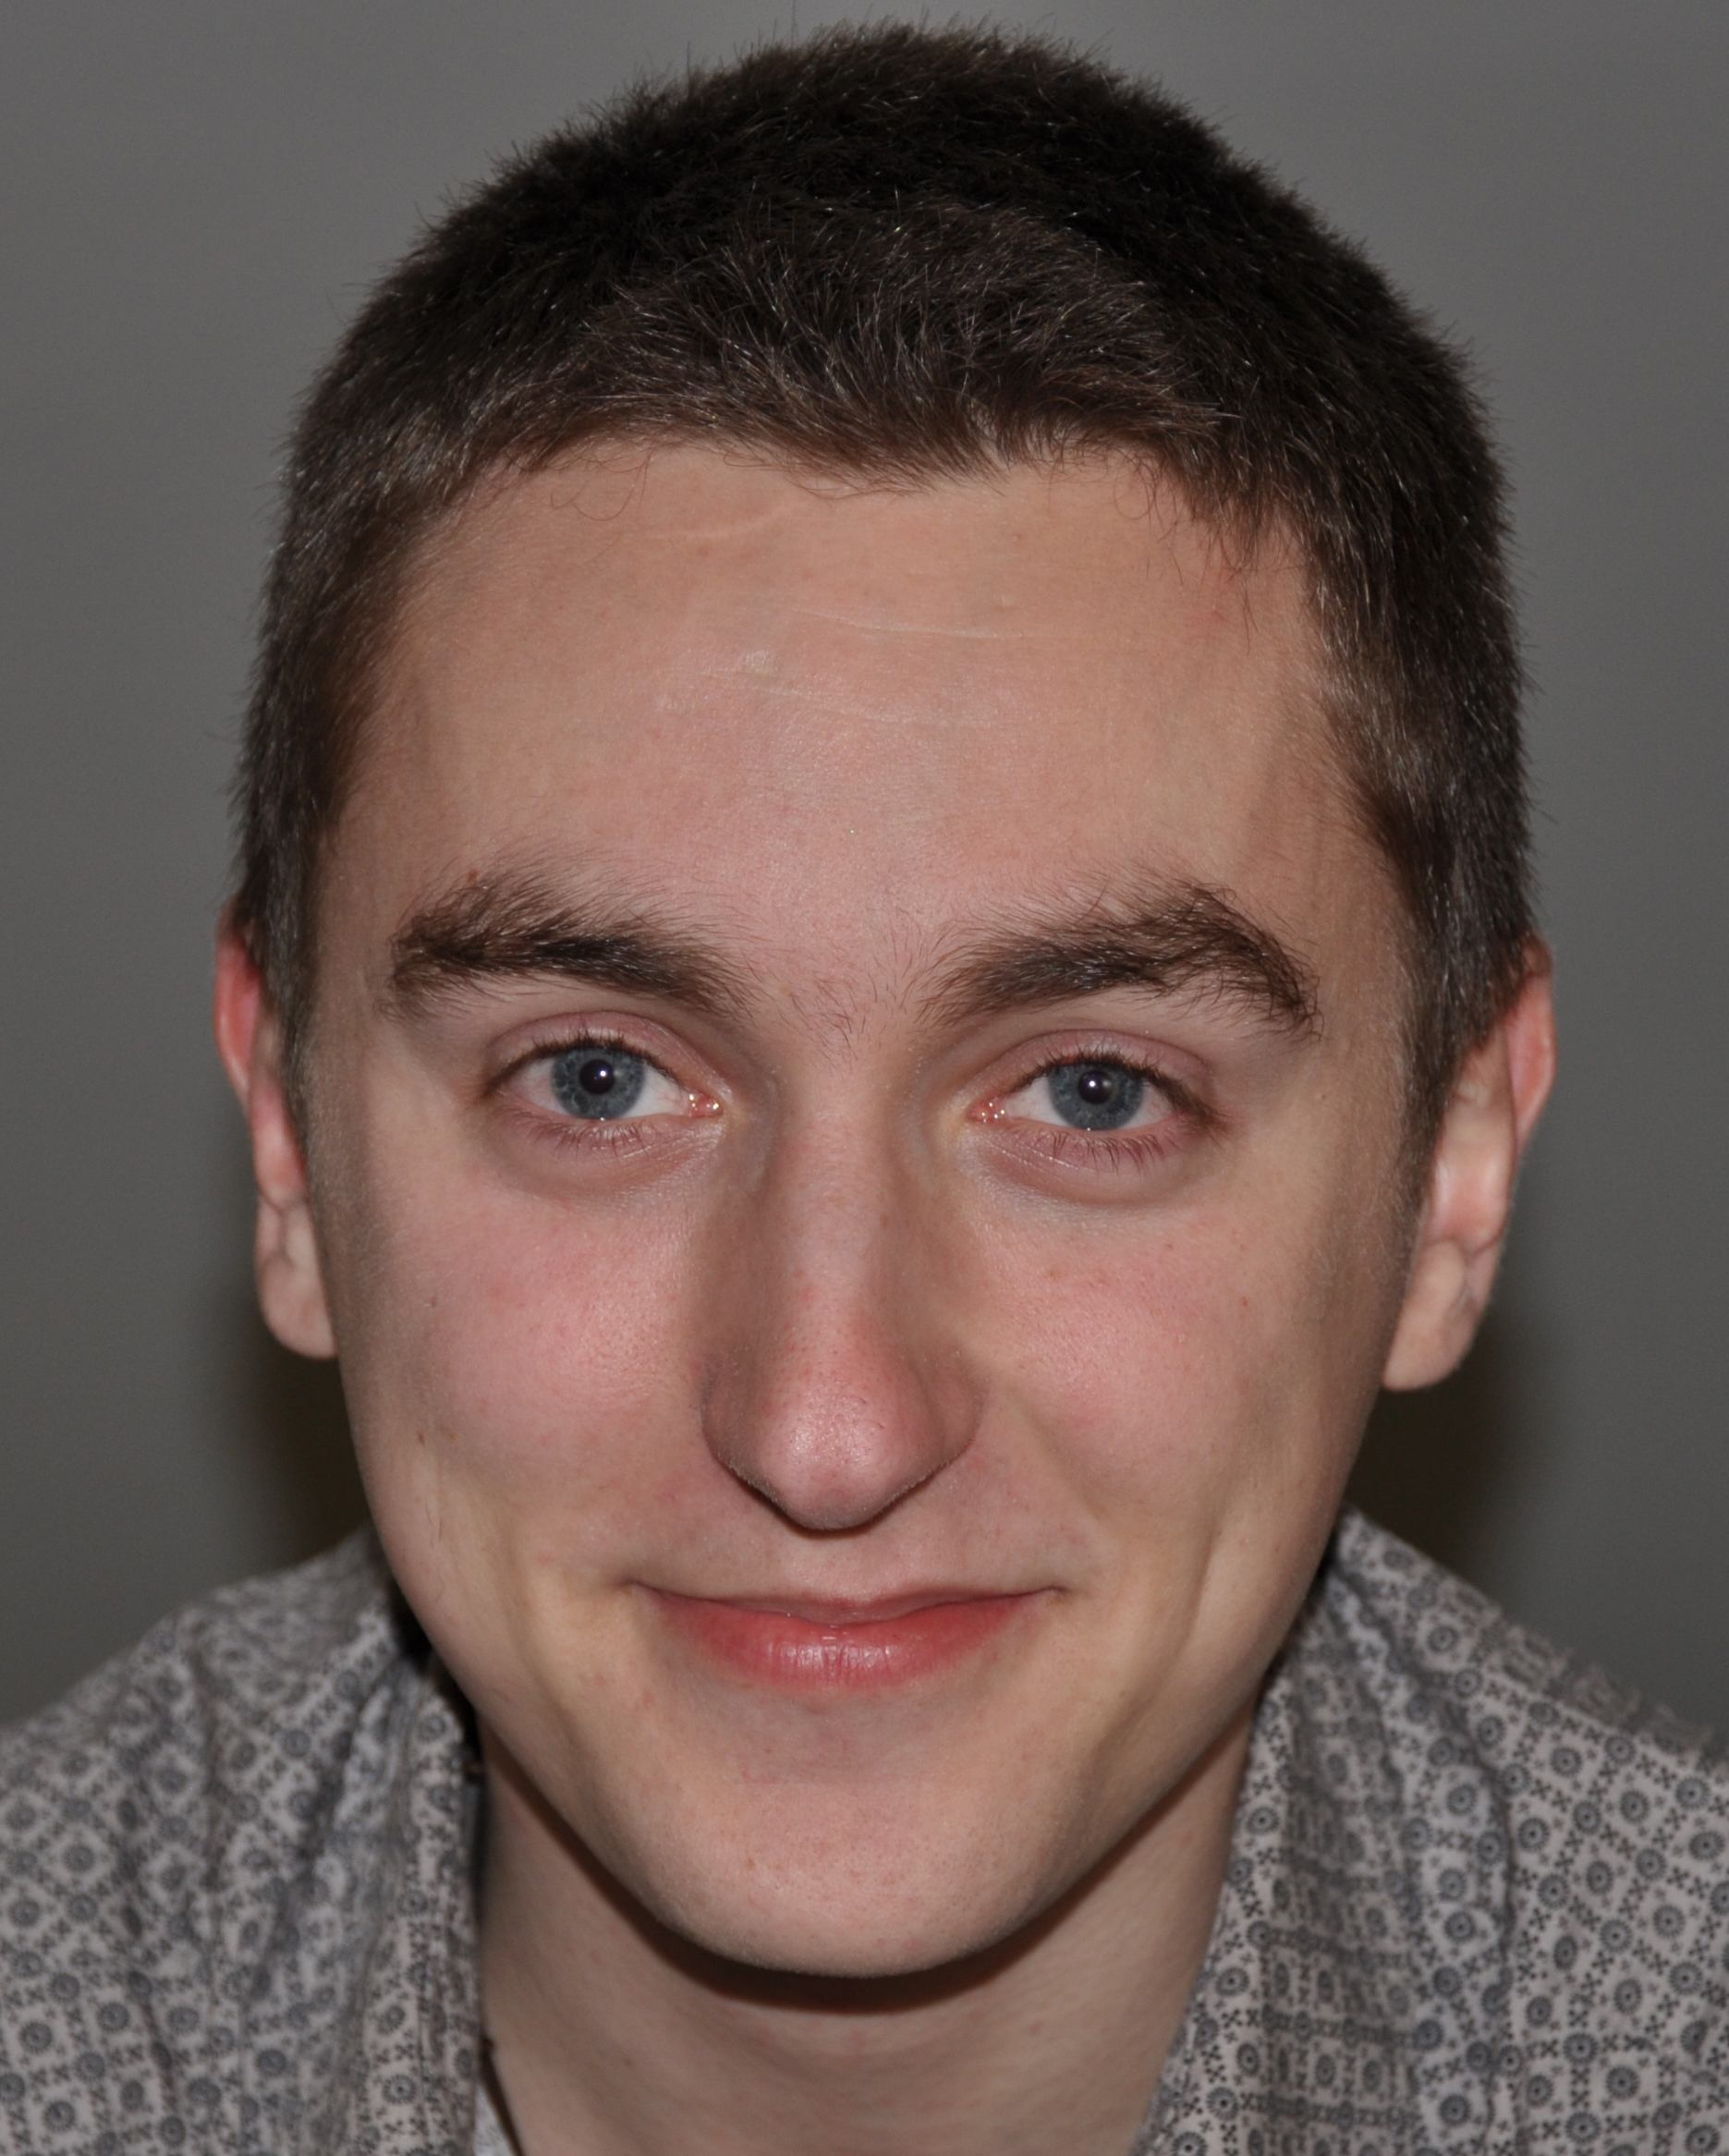
\includegraphics[scale=0.15]{Profil}
\section{Coordonnées}
Arnaud Bletterer
2, Route de Forstheim
67500 Haguenau
FRANCE
~
+333 69 02 09 52
+336 64 32 44 28
~
\href{mailto:arnaud.bletterer@gmail.com}{arnaud.bletterer@gmail.com}
\href{http://abletterer.fr}{http://abletterer.fr}
\section{Langues}
Français, langue natale
Anglais, niveau avancé
Allemand, niveau scolaire
\end{aside}

%----------------------------------------------------------------------------------------
%	EDUCATION SECTION
%----------------------------------------------------------------------------------------
\section{Formation}

\begin{entrylist}
%------------------------------------------------
\myentry
{2012-2014}
{Master {\normalfont Informatique, option Sciences de l'Image}}
{Université de Strasbourg, France}
%------------------------------------------------
\myentry
{2011-2012}
{Licence {\normalfont Informatique}}
{Université de Strasbourg, France}
%------------------------------------------------
\myentry
{2009-2011}
{Diplôme Universitaire de Technologie {\normalfont Informatique}}
{Université de Strasbourg, France}
%------------------------------------------------
\myentry
{2009}
{Baccalauréat {\normalfont Scientifique, Sciences de l'Ingénieur}}
{LEGTI Alphonse Heinrich, France}
%------------------------------------------------
\end{entrylist}

%----------------------------------------------------------------------------------------
%	WORK EXPERIENCE SECTION
%----------------------------------------------------------------------------------------

\section{Expérience}

\begin{entrylist}
%------------------------------------------------
\entry
{2014--6 mois}
{Stage de fin de Master}
{Equipe IGG, Laboratoire ICube, Strasbourg}
{Outils multidimensionnels de déformation \\ 
\underline{Références :} Dominique Bechmann, Isabelle Charpentier et Pierre Kraemer}
%------------------------------------------------
\entry
{2013--3 mois}
{Projet de développement logiciel}
{Université de Strasbourg}
{Génération de cage et déformation de l'espace \\ 
\underline{Références :} Dominique Bechmann et Pierre Kraemer}
%------------------------------------------------
\entry
{2013--3 mois}
{Travail d'étude et de Recherche}
{Université de Strasbourg}
{Multi-Triangulation\\\underline{Références :} Lionel Untereiner et Pierre Kraemer}
%------------------------------------------------
\entry
{2011--3 mois}
{Stage de fin de DUT}
{REP Solutions Interactive Inc., Québec, Canada}
{Développement d'applications côté client (JavaScript).\\
\underline{Référence :} Alain Marceau}
\end{entrylist}

%----------------------------------------------------------------------------------------
%	SKILLS SECTION
%----------------------------------------------------------------------------------------

\section{Compétences}

%------------------------------------------------
\textbf{Développement Web:}
PHP, HTML5, CSS3, Bootstrap, JavaScript, JQuery

%------------------------------------------------
\textbf{Génie Logiciel:}
C, C++, Java, C\#, SQL, MySQL, Oracle, PL/SQL, T-SQL, Merise, UML

%------------------------------------------------
\textbf{Systèmes:}
Linux, Windows, ShellScript, Systèmes distribués

%------------------------------------------------
\textbf{Synthèse d'Images:}
OpenGL, Cartes combinatoires, Déformation de maillages
%------------------------------------------------

%----------------------------------------------------------------------------------------
%	INTERESTS SECTION
%----------------------------------------------------------------------------------------

\section{Intérêts}

\textbf{Scientifiques:} Techniques de rendu, Maillages multirésolution

\textbf{Personnels:} Sport électronique, Athlétisme, Arts Martiaux, Guitare Basse

%----------------------------------------------------------------------------------------

\end{document}